\documentclass{beamer}
\usetheme[hideothersubsections]{HRTheme}
\usepackage{beamerthemeHRTheme}
\usepackage{graphicx}
\usepackage[space]{grffile}
\usepackage{listings}
\usepackage{animate}
\lstset{language=SQL,
basicstyle=\ttfamily\footnotesize,
mathescape=true,
keywordstyle=\color{blue},
breaklines=true,
showspaces=false,
showstringspaces=false}
\usepackage[utf8]{inputenc}
\usepackage{color}
\usepackage{multirow}
\newcommand{\red}[1]{
\textcolor{red}{#1}
}
\newcommand{\ts}{\textbackslash}

\title{ Crash recovery }

\author{ }

\institute{Hogeschool Rotterdam \\ 
Rotterdam, Netherlands}

\date{}

\begin{document}
\maketitle

\SlideSection{Introduction}
\SlideSubSection{Lecture topics}
\begin{slide}{
\item The log.
\item Analysis phase.
\item Redo phase.
\item Undo phase.
}\end{slide}

\SlideSection{Introduction to crash recovery}
\SlideSubSection{Transactions vs Crash recovery}
\begin{slide}{
	\item Transaction manager only grants \textit{Consistency} and \textit{Isolation} properties.
	\item We have not seen the case of an aborting transaction.
	\item If a transaction aborts we have to undo everything. This grants \textit{Atomicity}.
}\end{slide}

\SlideSubSection{Reasons}
\begin{slide}{
	\item We have to grant \textit{Consistency}.
	\item DBMS malfunctions after \texttt{Commit} operations.
	\item We have to redo everything the transaction committed.
}\end{slide}

\SlideSubSection{Cause of malfunctions}
\begin{slide}{
	\item Hardware failure
	\item Power grid failure
	\item Flooding
	\item Nuclear holocaust
	\item ...
	\item We must grant that the data is not lost
	
	\begin{figure}
		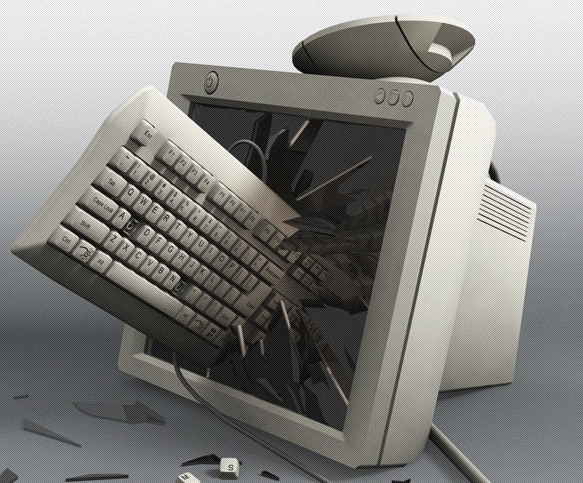
\includegraphics[scale=0.1]{img/hardware_failure}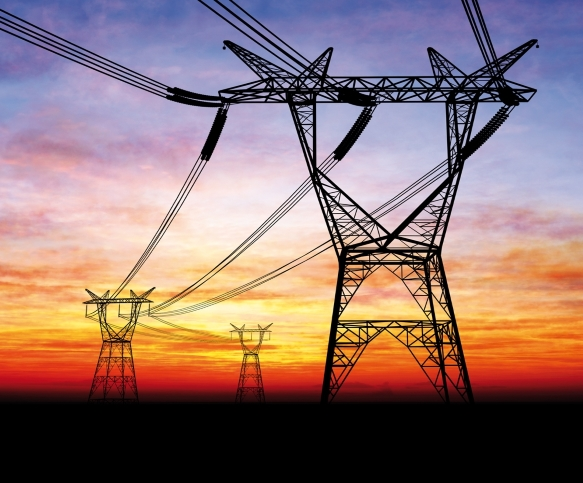
\includegraphics[scale=0.1]{img/power_grid}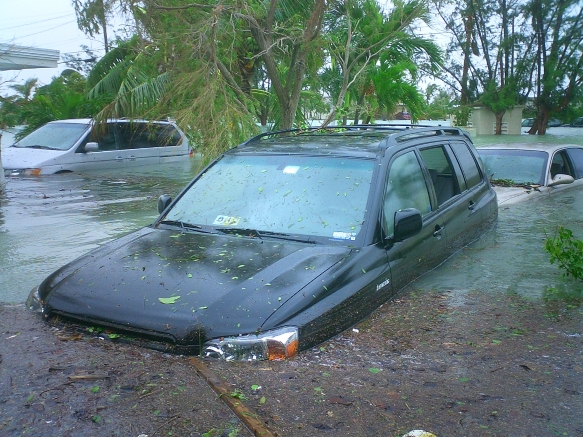
\includegraphics[scale=0.1]{img/flooding}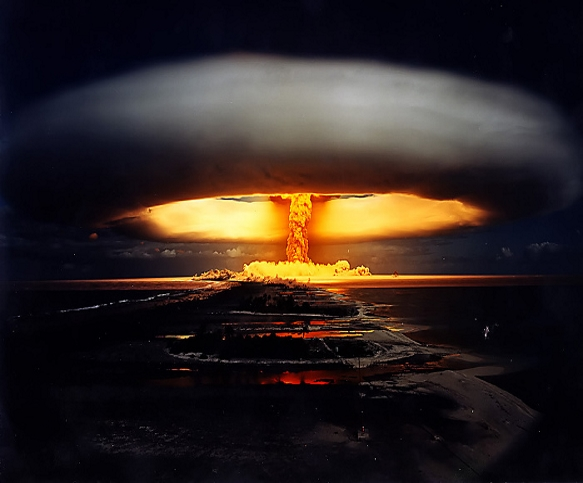
\includegraphics[scale=1]{img/nuclear_holocaust}
	\end{figure}
}\end{slide}

\SlideSection{ARIES}
\SlideSubSection{Overview}
\begin{slide}{
	\item Algorithm for crash recovery.
	\item Three phases:
	\begin{itemize}
		\item \textbf{Analysis:} tracks uncommitted data and active transactions during the crash.
		\item \textbf{Redo:} repeats all the actions to rebuild a valid state of the DB before the crash.
		\item \textbf{Undo:} cancel all the actions that were not committed at the crash.
	\end{itemize}
}\end{slide}

\SlideSubSection{Algorithm principles}
\begin{slide}{
	\item \textbf{Write-ahead logging:} keep track of the actions before you do them.
	\item \textbf{Repeating history: } After restarting retrace all the actions before the crash to bring back the DB to a consistent state.
	\item \textbf{Logging undo: } keep track of the undo actions before you do them (crash during restart).
}\end{slide}

\SlideSection{The log}
\SlideSubSection{Overview}
\begin{slide}{
	\item It is a history of the operations on the database.
	\item Each entry is called \textit{log record}.
	\item Each record contains a unique id (\textit{Log Sequence Number} - LSN), a type (kind of operation), and extra info.
	\item \textit{Log tail} partially maintained in main memory (RAM).
	\item Periodically stored into persistent memory.
}\end{slide}

\SlideSubSection{Update log record}
\begin{slide}{
	\item Used when a transaction modifies (i.e. writes) an object.
	\item Add the record to the log tail.
	\item The log record contains the transaction id, the object modified, the old value, and the updated value.
	\begin{table}
		\begin{tabular}{|c|c|c|c|c|c|}
			\hline
			\multicolumn{6}{|c|}{\textbf{Update}} \\
			\hline
			LSN & Type & TransID & Object & OldValue & NewValue \\
			\hline
		\end{tabular}
	\end{table}
}\end{slide}

\SlideSubSection{Commit log record}
\begin{slide}{
	\item Add the record to the log tail
	\item Force writing the log tail to permanent storage.
	\item The transaction is considered committed when the log tail is written successfully (handle crashes while writing the commit).
	\item The log record contains the transaction id that committed.
	\begin{table}
		\begin{tabular}{|c|c|c|}
			\hline
			\multicolumn{3}{|c|}{\textbf{Commit}} \\
			\hline
			LSN & Type & TransID \\
			\hline
		\end{tabular}
	\end{table}
}\end{slide}

\SlideSubSection{Abort log record}
\begin{slide}{
	\item Add the record to the log tail
	\item Start undo phase for that transaction (see slides about undo phase).
	\item The log record contains the transaction id that committed.
	\begin{table}
		\begin{tabular}{|c|c|c|}
			\hline
			\multicolumn{3}{|c|}{\textbf{Abort}} \\
			\hline
			LSN & Type & TransID \\
			\hline
		\end{tabular}
	\end{table}
}\end{slide}

\SlideSubSection{End log record}
\begin{slide}{
	\item Add the record to the log tail
	\item Written after extra actions of Commit or Abort are successfully executed.
	\begin{table}
		\begin{tabular}{|c|c|c|}
			\hline
			\multicolumn{3}{|c|}{\textbf{End}} \\
			\hline
			LSN & Type & TransID \\
			\hline
		\end{tabular}
	\end{table}
}\end{slide}

\SlideSubSection{Compensation log record}
\begin{slide}{
	\item Add the record to the log tail.
	\item Added after an undo operation is executed.
	\item It contains the type of the undo operation, and the LSN of the next record to be undone.
	\begin{table}
		\begin{tabular}{|c|c|c|c|}
			\hline
			\multicolumn{4}{|c|}{\textbf{CLR}} \\
			\hline
			LSN & Type & UndoType & NextLSN \\
			\hline
		\end{tabular}
	\end{table}
}\end{slide}

\SlideSubSection{Checkpoint}
\begin{slide}{
	\item Snapshot of the DBMS state.
	\item Used to reduce the amount of work during a restart.
	\item Insert a \textit{BeginCheckpoint} record in the log.
	\item Save the infos on active transactions and the dirty objects (i.e. written but uncommitted objects).
	\item Insert a \textit{EndCheckpoint} record in the log after this phase.
	\item Inexpensive: the system does not write the state, it writes the info to rebuild the state.
	\begin{table}
		\tiny
		\begin{tabular}{|c|c|}
			\hline
			\multicolumn{2}{|c|}{\textbf{BeginCheckpoint}} \\
			\hline
			LSN & Type \\
			\hline
		\end{tabular}
	\end{table}
	\begin{table}
		\tiny
		\begin{tabular}{|c|c|c|c|}
			\hline
			\multicolumn{4}{|c|}{\textbf{EndCheckpoint}} \\
			\hline
			LSN & Type & TransactionTable & DirtyObjects \\
			\hline
		\end{tabular}
	\end{table}
}\end{slide}

\SlideSubSection{Logging active transactions}
\begin{slide}{
	\item \textbf{Transaction id: } the name of the transaction.
	\item \textbf{LastLSN}: the LSN of the most recent log for this transaction.
	\item \textbf{Status}: In progress (P), Committed (C), or Undone (U).
}\end{slide}

\SlideSubSection{Logging dirty objects}
\begin{slide}{
	\item \textbf{Object id: } The name of the modified object/variable.
	\item \textbf{RecLSN}: LSN of the first record that caused the object to become dirty.
	\item If possible (only if committed) the DBMS periodically writes to disk the dirty objects.
	\item When the objects are written to the disk they are removed from the table.
}\end{slide}

\SlideSubSection{Example}
\begin{slide}{
	\item Consider the execution of operations on the database below and the initial state below.
	\item Write the log that must be created for that execution to support crash recovery.
	
	\begin{table}
		\tiny
		\begin{tabular}{|c|c|}
			\hline
			\textbf{Variable} & \textbf{Value} \\
			\hline
			A & 2\\
			\hline
			B & 0 \\
			\hline
		\end{tabular}
	\end{table}
	\begin{table}
		\tiny
		\begin{tabular}{|c|c|}
			\hline
			\textbf{Time} & \textbf{Operation} \\
			\hline
			16:00 PM & T1 writes A + 1 \\
			\hline
			16:01 PM & T2 writes B + 5 \\
			\hline
			16:02 PM & Checkpoint \\
			\hline
			16:03 PM & Commit T1\\
			\hline
			16:05 PM & T2 writes A + 3 \\
			\hline
			16:06 PM & T2 writes B - 2 \\
			\hline
			16:07 PM & Commit T2\\
			\hline
		\end{tabular}
	\end{table}
}\end{slide}

\SlideSubSection{Example}
\begin{slide}{
	\item The following is the created log:
	
	\begin{table}
		\tiny
		\begin{tabular}{|c|c|c|c|c|c|}
			\hline
			0 & Update & T1 & A & 2 & 3 \\
			\hline
			1 & Update & T2 & B & 0 & 5 \\
			\hline
			2 & BeginCheckpoint & \multicolumn{4}{}{} \\
			\cline{1-4}
			3 & EndCheckpoint & (T1,0,P),(T2,1,P) & (A,0),(B,1) & \multicolumn{2}{}{} \\
			\cline{1-4}
			4 & Commit & T1 & \multicolumn{3}{}{} \\
			\cline{1-3}
			5 & End & T1 & \multicolumn{3}{}{} \\
			\hline
			6 & Update & T2 & A & 3 & 6 \\
			\hline
			7 & Update & T2 & B & 0 & 3 \\
			\hline
			8 & Commit & T2 & \multicolumn{3}{}{} \\
			\cline{1-3}
			9 & End & T2 & \multicolumn{3}{}{} \\
			\cline{1-3}
		\end{tabular}
	\end{table}
}\end{slide}

\SlideSubSection{Assignment}
\begin{slide}{
	\item Consider the execution of operations on the database below and the initial state below.
	\item Write the log that must be created for that execution to support crash recovery.
	
	\begin{table}
		\tiny
		\begin{tabular}{|c|c|}
			\hline
			\textbf{Variable} & \textbf{Value} \\
			\hline
			A & 2\\
			\hline
			B & 0 \\
			\hline
			C & 3 \\
			\hline
		\end{tabular}
	\end{table}
	\begin{table}
		\tiny
		\begin{tabular}{|c|c|}
			\hline
			\textbf{Time} & \textbf{Operation} \\
			\hline
			10:00 AM & T1 writes A - 5 \\
			\hline
			10:02 AM & T2 writes B + 3 \\
			\hline
			10:03 AM & Commit T1 \\
			\hline
			10:05 AM & T2 writes A + 2\\
			\hline
			10:06 AM & T3 writes C - 4 \\
			\hline
			10:10 AM & T2 writes A + 1\\
			\hline
			10:12 AM & Checkpoint \\
			\hline
			10:14 AM & T2 Commit \\
			\hline
			10:20 AM & T3 writes A + 3 \\
			\hline
			10:21AM & T3 writes C + 2 \\
			\hline
			10:22AM & T3 Commit \\
			\hline
		\end{tabular}
	\end{table}
}\end{slide}

\SlideSection{Crash recovery}
\SlideSubSection{Analysis phase}
\begin{slide}{
	\item We need a point in the log to start from.
	\item The latest checkpoint is the point where we could have a valid state of the DBMS.
	\item Start from the latest checkpoint.
	\item Scan forward the log.
	\item From simplicity we assume that no record is written between the start and end checkpoint logs (the operation is atomic and never fails).
}\end{slide}

\SlideSubSection{Analysis phase}
\begin{slide}{
	\item If we find an end log for T, we remove T from the active transactions
	\item If we find a log record different from an end log, we add transaction T to the active transactions if not there.
		\begin{itemize}
			\item Set \texttt{LastLSN} for T to be the current LSN.
			\item If the log record is a Commit change the state into C, otherwise into U.
		\end{itemize}
	\item If we find an update log affecting object A, and A is not among the dirty objects, we add A to the dirty object and set \texttt{RecLSN} to the current LSN.
}\end{slide}

\SlideSubSection{Example}
\begin{slide}{
	\item Given the log below, show the active transaction table, and the dirty object table after analysing each log record.
	
	\begin{table}
		\tiny
		\begin{tabular}{|c|c|c|c|c|c|}
			\hline
			0 & Update & T1 & A & 2 & 3 \\
			\hline
			1 & Update & T2 & B & 0 & 5 \\
			\hline
			2 & BeginCheckpoint & \multicolumn{4}{}{} \\
			\cline{1-4}
			3 & EndCheckpoint & (T1,0,P),(T2,1,P) & (A,0),(B,1) & \multicolumn{2}{}{} \\
			\cline{1-4}
			4 & Commit & T1 & \multicolumn{3}{}{} \\
			\cline{1-3}
			5 & End & T1 & \multicolumn{3}{}{} \\
			\hline
			6 & Update & T2 & C & -1 & 6 \\
			\hline
			7 & Update & T2 & D & 1 & 3 \\
			\hline
			\multicolumn{6}{|c|}{Crash, restart} \\
			\hline
		\end{tabular}
	\end{table}
}\end{slide}

\SlideSubSection{Example}
\begin{slide}{
	\item The follwing tables are the active transaction table and the dirty object table at each step:
	
	\begin{table}
		\tiny
		\begin{tabular}{|c|c|c|c|}
			\hline
			\multicolumn{4}{|c|}{\textbf{Active transactions}} \\
			\hline
			\textbf{LSN} & TransactionId & LastLSN & Status \\
			\hline
			\multirow{2}{*}{4} & T1 & 4 & C \\
			& T2 & 4 & P \\
			\hline
			5 & T2 & 5 & P \\ 
			\hline
			6 & T2 & 6 & P \\
			\hline
			7 & T2 & 7 & P \\
			\hline
		\end{tabular}
	\end{table}
	
	\begin{table}
		\tiny
		\begin{tabular}{|c|c|c|}
			\hline
			\multicolumn{3}{|c|}{\textbf{Dirty Objects}} \\
			\hline
			\textbf{LSN} & Object & RecLSN \\
			\hline
			\multirow{2}{*}{4 - 7} & A & 0 \\
			& B & 1 \\
			\hline
			\multirow{2}{*}{6 - 7} & A & 0 \\
			& B & 1 \\
			& C & 6 \\
			& D & 7 \\
			\hline
		\end{tabular}
	\end{table}
}\end{slide}

\SlideSubSection{Redo Phase}
\begin{slide}{
	\item Redo all the updates of all the transactions in the active transaction table.
	\item Find the smallest among all RecLSN of all the objects.
	\item This phase redoes also all the CLR's (see undo phase).
	\item In this phase we assume that we maintain a ObjectLSN used after each redo operation on an object. 
}\end{slide}

\SlideSubSection{Redo Phase}
\begin{slide}{
	\item Each action must be redone unless one of the following rules is satisfied:
	\begin{enumerate}
		\item The affected object is not dirty.
		\item The affected object is dirty, but RecLSN is greater than the LSN of the current log record.
		\item The ObjectLSN is greater than or equal to the LSN of the log record.
	\end{enumerate}
}\end{slide}

\SlideSubSection{Redo Phase: Rule 1}
\begin{slide}{
	\item The first rules means that the object has been written to disk.
	\item It happens when there is a crash after a checkpoint and the object was added in the dirty object table at that checkpoint.
	\item The page might have been written to disk but we have gone back before the checkpoint.
}\end{slide}

\SlideSubSection{Redo Phase: Rule 2}
\begin{slide}{
	\item The first rule means that the object is still in the dirty object table but it was later written to disk.
	\item It happens when there is a crash after a checkpoint and the object was added in the dirty object table at that checkpoint.
	\item The page might have been written to disk but we have gone back before the checkpoint.
}\end{slide}

\SlideSubSection{Redo Phase: Rule 3}
\begin{slide}{
	\item The third rule requires to access the dirty object table
	\item It might happen when there is a crash during a redo phase which successfully redid some of the operations.
	\item This condition alone is sufficient also for rules 1 and 2.
	\item It is an expensive operations because we have to access to the disk. Better check also rule 1 and rule 2 that do not require this.
}\end{slide}

\SlideSubSection{Redo Phase: redoing operations}
\begin{slide}{
	\item The logged operation is re-applied.
	\item The ObjectLSN is set to the LSN of the log record that was re-applied.
}\end{slide}

\SlideSubSection{Example}
\begin{slide}{
	\item Given the log used in the analysis phase and the generated tables, determine the log from which the redo phase start and what operations are affected. Motivate the answer.
		
	\vspace{1cm}
	\item The smallest RecLSN = 6.
	\item The update on C is redone, because SLN $\leq$ RecLSN.
	\item The update on D is redone, same reason.	
}\end{slide}

\SlideSubSection{Undo Phase}
\begin{slide}{
	\item Start from the transaction with largest LastLSN.
	\item For each transaction do the following
	\begin{itemize}
		\item Write a CLR setting NextLSN to the LSN of the action of the operation on this transaction before this log record.
		\item If it does not exist, set it to \texttt{null}.
		\item Undo the operation.
	\end{itemize} 
	\item If the action is a CLR:
		\begin{itemize}
			\item if NextSLN is not \texttt{null}, repeat the undo on that operation.
			\item if it is \texttt{null} add an end record for the transaction because it has completely undone.
		\end{itemize}
}\end{slide}

\SlideSubSection{Aborting transactions}
\begin{slide}{
	\item Aborting transactions is just like a system crash.
	\item Consider the entries in the table just for the aborting transaction.
	\item Apply the undo phase for that transaction.
}\end{slide}

\SlideSubSection{Assignment}
\begin{slide}{
	\item Using the log and the tables built in the analysis phase, write an updated log by inserting the appropriate CLR added during the Undo phase.
}\end{slide}


\end{document}